\section{Transformers}

\subsection{Self-attention}

Let $\mat{X} \in \R^{T \times d}$ denote the input embeddings and $\mat{\Xi} \in \R^{T \times d_v}$
the output embeddings. The problem with $\mat{X}$ is that the embeddings are non-contextual---each
embedding has no information about its neighbors. Self-attention aims to contextualize the
embeddings in $\mat{\Xi}$.

It does so by computing queries, keys, and values by linear projections of the input, \[
    \mat{Q} = \mat{X} \mat{W}_Q, \quad \mat{K} = \mat{X} \mat{W}_K, \quad \mat{V} = \mat{X} \mat{W}_V,
\]
where $\mat{W}_Q, \mat{W}_K \in \R^{d \times d_k}$ and $\mat{W}_V \in \R^{d \times d_v}$.
Intuitively, for each timestep, the queries represent what information is missing, the keys
represent the information that is offered, and the values are the actual information.

The attention mechanism is computed as follows, \[
    \mat{A} = \mathrm{softmax}\lft( \frac{\mat{Q} \transpose{\mat{K}}}{\sqrt{d_k}} \rgt), \quad \mat{\Xi} = \mat{A} \mat{V}. \margintag{Softmax is performed row-wise. The division by $\sqrt{d_k}$ is necessary because $\Var[\vec{x} \cdot \vec{y}] = d$, where $\vec{x}, \vec{y} \sim \mathcal{N}(\vec{0}, \mat{I}_d)$. We want to recover unit variance.} \\
\]
Here, $\mat{A} \in \R^{T\times T}$ is the attention matrix---$\vec{a}_i$ is a convex combination
that tells us how much attention the $i$-th timestep pays to each other timestep. The rank of this
matrix is bounded by $d_k$.

The contextualized outputs are convex combinations of values, \[
    \vec{\xi}_i = \sum_{t=1}^{T} \mathrm{softmax}_t(\vec{a}_i) \vec{v}_i, \quad a_{it} \propto \transpose{\vec{q}_i} \vec{k}_t.
\]
This makes intuitive sense, because the weight of the $t$-th timestep for timestep $i$ depends on
the alignment between $\vec{q}_i$ and $\vec{k}_t$. Furthermore, $\vec{\xi}_i$ depends only on its
corresponding query and all other key-value pairs. In a sense, the attention mechanism is a
soft-dictionary lookup.

\begin{marginfigure}
    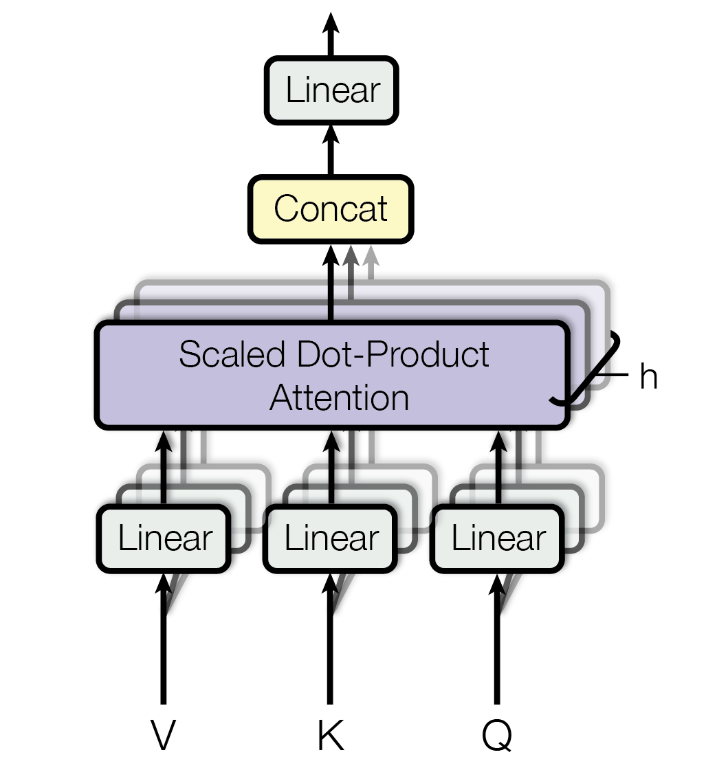
\includegraphics[width=\textwidth]{figures/mhsa}
    \caption{Multi-headed self-attention \citep{vaswani2017attention}.}
    \label{fig:mhsa}
\end{marginfigure}

MHSA (\textit{\textbf{M}ulti-\textbf{H}eaded \textbf{S}elf-\textbf{A}ttention}) computes multiple
attention mechanism in parallel---see \Cref{fig:mhsa}. Let $h$ be the number of heads, then we
first compute $h$ queries, keys, and values for each input token.\sidenote{In practice, we use
    three---not $3 \cdot h$---linear layers for the query, key, and value representations, where the
    output is $h \cdot d_k$-dimensional. We can chunk this output to get the corresponding
    representations for each head. This makes PyTorch---or any other library---compute the heads in
    parallel.} Then, we apply attention $h$ times using these representations and concatenate the
outputs into a single vector. Lastly, we perform a linear layer to combine the outputs of the
heads.

\subsection{Cross-attention}

A cross-attention layer takes two sequences as inputs, \[
    \mat{A} \in \R^{T_a \times d_a}, \quad \mat{B} \in \R^{T_b \times d_b}.
\]
Then, it computes the queries from $\mat{A}$ and the keys and values from $\mat{B}$, \[
    \mat{Q} = \mat{A} \mat{W}_Q, \quad \mat{K} = \mat{B} \mat{W}_K, \quad \mat{V} = \mat{B} \mat{W}_V,
\]
where $\mat{W}_Q \in \R^{d_a \times d_k}$, $\mat{W}_K \in \R^{d_b \times d_k}$, and $\mat{W}_V \in
    \R^{d_b \times d_v}$. Then, we can apply (multi-headed) attention to these representations. This is
an effective way of giving additional sequence data $\mat{B}$ to a sequence $\mat{A}$.

\subsection{Positional encoding}

The attention mechanism is permutation equivariant, which means that the order of input tokens does
not influence the output. So, we need a way of reintroducing the sequence structure to this
mechanism. We do this by defining a positional encoding matrix $\mat{P} \in \R^{T \times d}$ and
adding it to the input sequence, $\mat{X} + \mat{P}$. A common way of defining this matrix is as
follows, \[
    p_{tk} =
    \begin{cases}
        \sin(t \omega_k) & k \mod 2 = 0  \\
        \cos(t \omega_k) & k \mod 2 = 1,
    \end{cases}
    \quad
    \omega_k \doteq C^{\nicefrac{k}{d}}. \margintag{$C=10^4$.}
\]
A heatmap representation of this matrix can be seen in \Cref{fig:pe}.

\begin{marginfigure}
    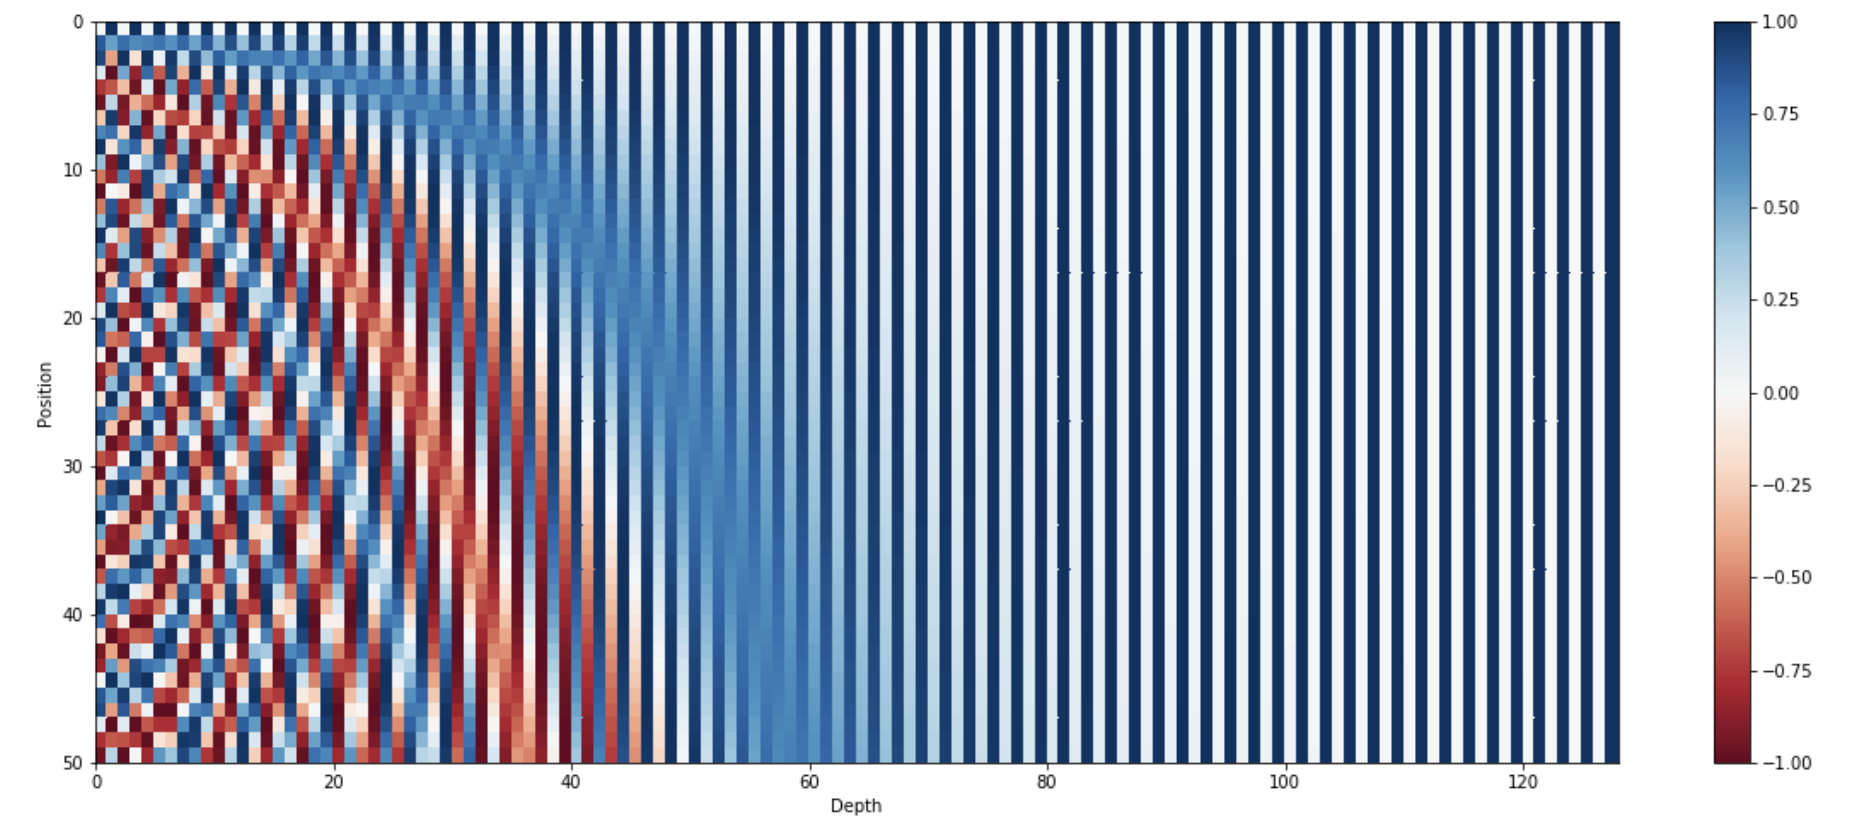
\includegraphics[width=\textwidth]{figures/positional-encoding}
    \caption{Positional encoding matrix, represented as a heatmap.}
    \label{fig:pe}
\end{marginfigure}

\subsection{Machine translation}

The transformer \citep{vaswani2017attention} was the first architecture to show that attention can
be used effectively in machine learning. \citet{vaswani2017attention} designed an encoder and an
autoregressive decoder for machine translation---see \Cref{fig:transformer-arch}. The encoder works
by applying an MHSA layer and a pointwise MLP layer $N$ times in an alternating fashion. In
addition, it also employs residual connections \citep{he2016deep} and layer normalization
\citep{lei2016layer}. These are essential for effectively backpropagating gradients and ensuring
stability. Furthermore, it also makes use of positional encoding to preserve order information. Let
$\mat{X} \in \R^{T \times d}$ denote the input of the encoder and $\mat{\Xi} \in \R^{T \times d}$
its output.

\begin{marginfigure}
    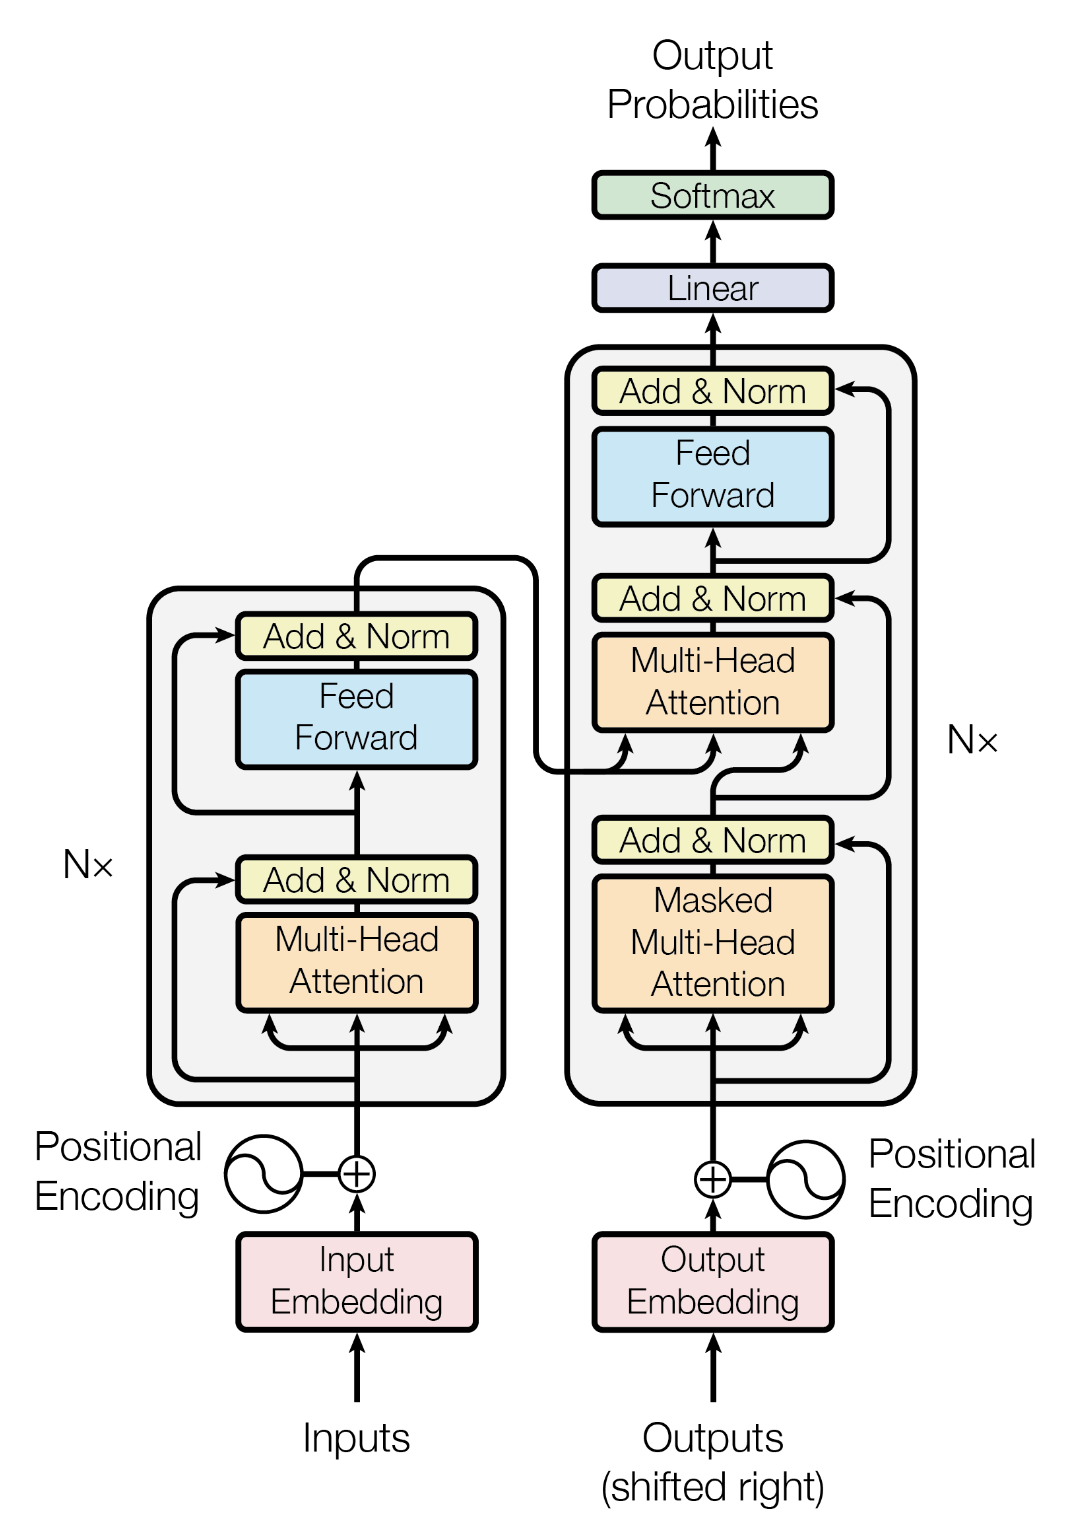
\includegraphics[width=\textwidth]{figures/transformer-architecture}
    \caption{Architecture of the transformer \citep{vaswani2017attention}. The left side is called the encoder, which encodes the input sentence. The right side is called the decoder, which uses cross-attention to incorporate information from the source sequence in the prediction of the target sequence. The model works in an autoregressive manner, which means that the next token is predicted from the history until an end-of-sentence token is predicted.}
    \label{fig:transformer-arch}
\end{marginfigure}

Furthermore, the decoder works in an autoregressive manner, which means that it computes the output
tokens one-by-one. The decoder first receives the history of previously generated tokens
$\mat{Y}_{1:t-1}$ and contextualizes it using an MHSA layer. Let $\mat{\Upsilon}_{1:t-1}$ denote
the output of the MHSA layer. Then, a multi-headed cross-attention layer receives $\mat{\Xi}$ as
input and aligns $\mat{\Upsilon}_{1:t-1}$ with it. Lastly, a pointwise MLP is applied. It performs
these steps $N$ times. Again, the decoder makes use of residual connections and layer normalization
to ensure stability of the gradient and output.

The advantage of this architecture is that---unlike RNNs---we do not need to memorize tokens in the
hidden state, because we can look back at the full sequence at every step. However, this has the
disadvantage that we need to look at the full sequence at every step, instead of having all
information encoded in a precomputed hidden state. Furthermore, transformers allow for easy scaling
up by simply increasing the number of heads, hidden dimensionality, or the number of
encoders/decoders.

\subsection{BERT}

BERT (\textit{\textbf{B}idirectional \textbf{E}ncoder \textbf{R}epresentations from
    \textbf{T}ransformers}) \citep{devlin2018bert} is a transformer-based pretrained LM that can be
used for finetuning on downstream natural language processing tasks. BERT first tokenizes its input
sequence using WordPiece tokenization \citep{wu2016google} and prepends it with a \texttt{[CLS]}
token. Further, it makes use of the encoder blocks from the transformer architecture to
contextualize its input tokens. When the weights of these encoders are pretrained, we can place
additional layers on top of the encoders that operate on BERT's contextualized tokens. We then
finetune the weights of the full model on the specific task we are interested in.

BERT's pre-training consists of two stages,
\begin{enumerate}
    \item \textit{Predicting masked out tokens using its left and right context as input.}\sidenote{This is also known
              as the Cloze test \citep{taylor1953cloze}. Cloze tests require the ability to understand the
              context and vocabulary in order to identify the correct language or part of speech that belongs in
              the deleted passages.}\sidenote{BERT masks 15\% of tokens, of which 80\% is replaced by
              \texttt{[MASK]}, 10\% is replaced by a random token, and 10\% is left unchanged.} The
          task is performed by passing a masked out text to BERT to retrieve its representations.
          Then, the representation embedding of the masked tokens are passed to a model that predicts which token
          was originally there. This was previously not easy to do with RNNs, because they can
          only process sequences left-to-right or right-to-left;
    \item \textit{Binary next sentence classification, where the model must classify two sentences as being
              consecutive or not.} Here, the two sentences are separated by a \texttt{[SEP]}-token as input to BERT.
          In order to make classification possible, the \texttt{[CLS]}-token is appended to the
          input tokens and its representation is used for the final prediction network.
\end{enumerate}
The first stage trains BERT's understanding of language, whereas the second stage enables BERT to infer relationships
between sentences, which is important for tasks like question-answering.

Lastly, we can finetune the parameters of BERT with a small ground truth dataset to a large variety
of tasks. \Eg,
\begin{itemize}
    \item \textit{Question answering}, where a question and a context passage is provided with a \texttt{[SEP]}-token
          separating them. Each token is passed to start and end token classifiers, which predict how likely
          each token is to be the start and end of the answer. Using these classifiers, we can extract the
          answer from the passage;
    \item \textit{Part-of-speech tagging}, where each token embedding is passed to a classification model, which
          outputs a distribution over part-of-speech tags;
    \item \textit{Sentiment classification}, where the representation of the \texttt{[CLS]}-token is passed to a
          binary classification model that predicts whether the sentence is positive or negative.
\end{itemize}

\subsection{Vision transformer}

ViT (\textit{\textbf{Vi}sion \textbf{T}ransformer}) \citep{dosovitskiy2020image} adapts the
transformer architecture to images by treating patches of an input image as its tokens---see
\Cref{fig:vit}. \citet{dosovitskiy2020image} showed the effectiveness of this approach by adapting
the transformer architecture to an image classification task. ViT computes the input tokens by
vectorizing $16 \times 16$ patches of the input image and linearly projecting them to a token
space. Further, a \texttt{[CLS]}-token is prepended to the sequence of tokens. Then, ViT employs
the encoder architecture of the transformer to contextualize its input representations. Finally,
the contextualized embedding of the \texttt{[CLS]}-token is passed to a classification network that
predicts the class of the input image.

\begin{figure}[t]
    \centering
    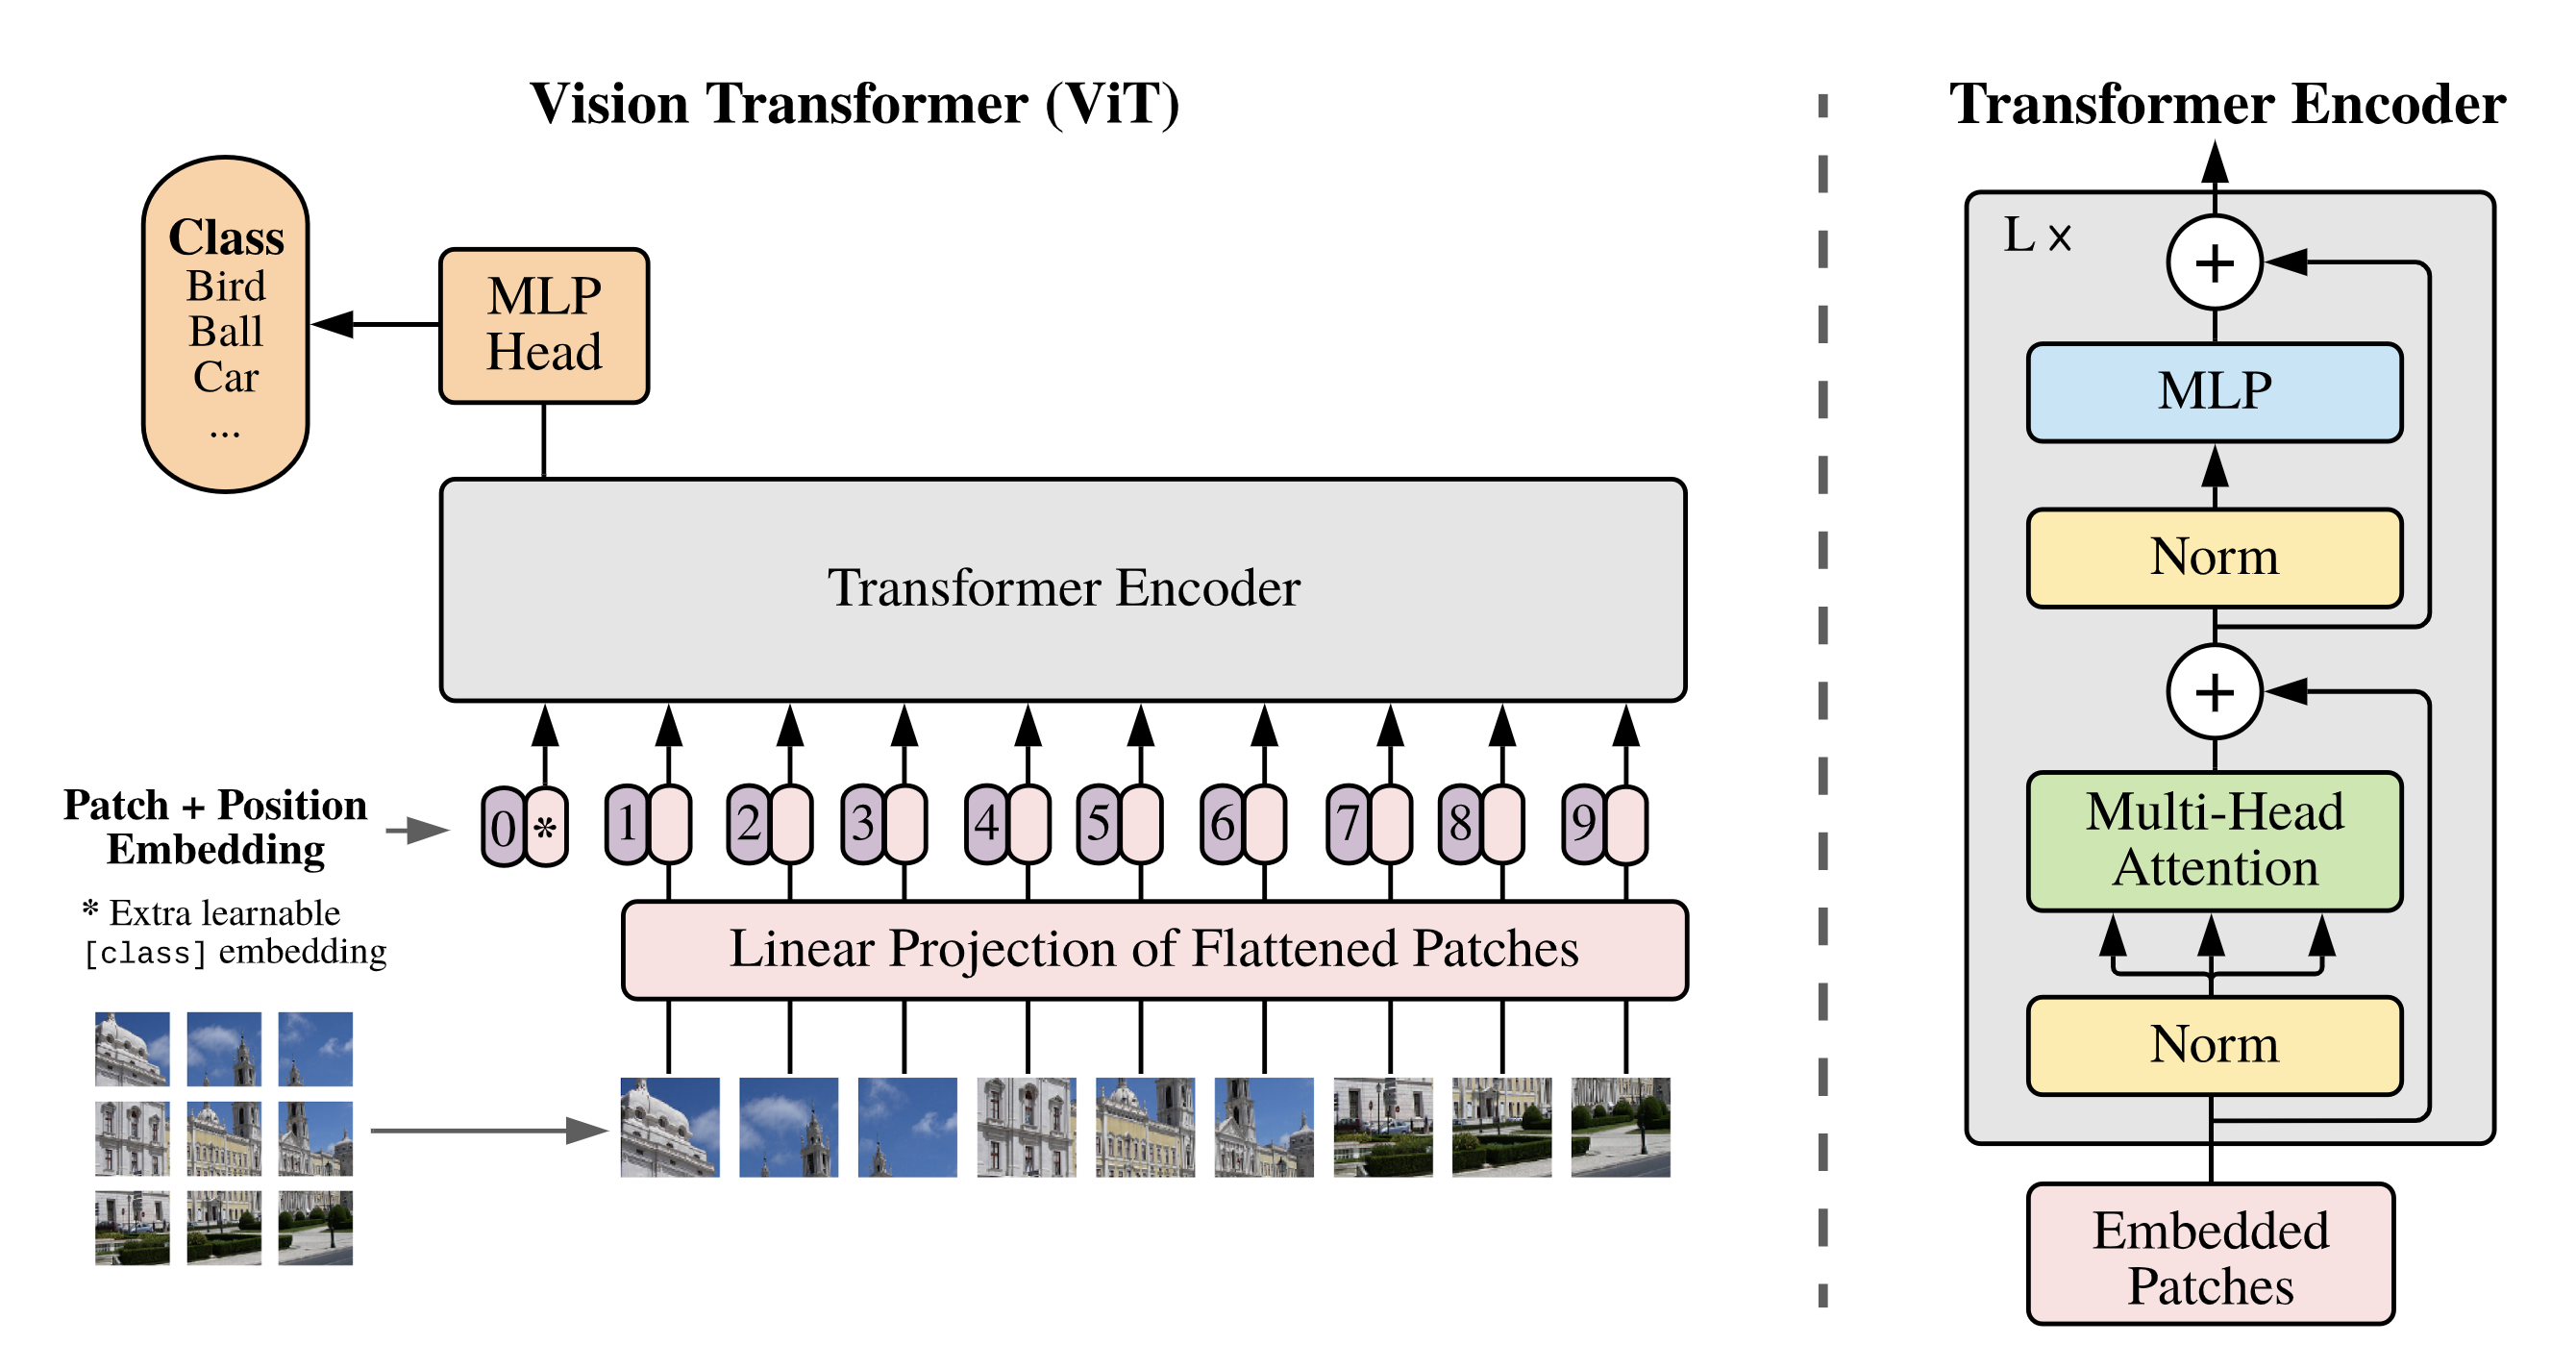
\includegraphics[width=\textwidth]{figures/vit}
    \caption{Architecture of the vision transformer \citep{dosovitskiy2020image}.}
    \label{fig:vit}
\end{figure}

A possible reason for this model's effectiveness is that this architecture carries less inductive
bias than CNN-based models. In general, this seems to be beneficial for very large datasets.
